\section{Prozesse}

\subsection{Bestandteile}
\begin{itemize}
    \item eigener Adressraum
    \item Programmcode
    \item Programmdaten
    \item Programm-Counter
    \item Stacks und Stackpointer
    \item Hardwareregister-Inhalte \textit{(Prozess-Kontext)}
    \item Heap-Speicher
    \item Verwaltungsdaten
    \begin{itemize}
        \item Identifier und VaterID
        \item Resourcenliste
        \item Scheduling Parameter
    \end{itemize}
\end{itemize}

\begin{figure}[ht!]
    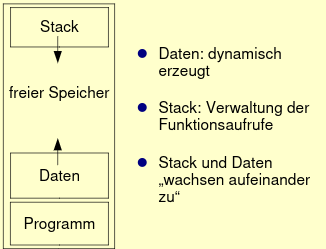
\includegraphics[scale=.75]{pics/processes}
    \caption{Process Control Block PCB}
\end{figure}

\subsection{Hierarchie und Signale}
Jeder Prozess hat \textbf{Vaterprozess} \textit{(Prozesse erzeugen einander)}.

\subsubsection{Signale}
\begin{itemize}
    \item (17) STOP \textit{(Strg-Z oder bg)}
    \item (19) CONT \textit{(fg)}
    \item (15) SIGTERM \textit{(beenden)}
    \item (9) KILL \textit{(abschließen)}
\end{itemize}